\chapter{Related Work} \label{chap:Chapter3}       
\epigraph{``This is where technology is now, imagine where we can go in the future” }{\textit{Timothy Chung}}

Σε αυτό το \emph{Chapter} περιγράφονται τρόποι - από την βιβλιογραφία - με τους οποί\-ους, οι υπάρχουσες εφαρμογές 
από drone swarms επιλύουν το localization pro\-blem. Κάποια από τα συστήματα στις υπάρχουσες έρευνες\udot έχουν καθαρά
θεωρητική πλευρά, άλλα έχουν δοκιμαστεί σε real-life scenarios.
Ενώ, σε αρκετές από αυτές τις εφαρμογές χρησιμοποιούνται - 
και για αυτό γίνεται αναφορά - τεχνικές που αναφέ\-ρθηκαν στο \emph{Chapter} \ref{chap:Chapter2}.

Πρώτο πράγμα που πρέπει να σκεφτούμε είναι ότι 

Πριν αναφερθούν 
Local Positioning System (LPS)
flying ad-hoc network (FANET)

Λίγα λόγια πριν για φίλτρα κλπ

important cordinate frames
LPS-coordinate frame and
the UAV body frame is obtained

- ραδιο 
	μικρη αναφορά στα παπερς και μετά ένα ένα λίγα πράγματα

- ήχος

- εικόνα

Extended Kalman Filter

% ------------------------------------------------------------------------------------
\section{Radio}


Πρώτη αναφορά \cite{uwb-imu-gps1} \cite{uwb-imu-gps2} \cite{uwb-imu-gps3}
Ultra-Wideband Based Pose Estimation for SmallUnmanned Aerial Vehicles

Cooperative 3-D relative localization for UAV swarm by fusing UWB withIMU and GPS

Accurate  3D  Localization  for  MAV  Swarms  by  UWB  and  IMU  Fusion

\subsection{UWB, IMU and GPS}
Στο \cite{uwb-imu-gps1}, υπάρχουν Ν αριθμημένα drones, θεωρώντας την λογική του γράφου - για την αναπαράσταση των nodes - οπως 
περιγράφτηκε στο προηγούμενο κεφάλαιο. Ενώ κάθε node περιλαμβάνει IMU/Compass/GPS και Αltitude and Heading Reference 
System(AHRS) που αξιοποιείται από ένα flight control unit, με την χρήση των οποίων μπορούν σε NED coordinate frame (N frame) να συλλέξουν πληροφορίες όπως παρουσιάζονται 
στους παρακάτω πίνακες για κάθε timeframe Κ.

\begin{gather*}
	\textbf{GPS Position:}\quad r^k_{i, GPS} = \left[x^k_{i, GPS} \quad y^k_{i, GPS} \quad z^k_{i, GPS}\right]^T \\
	\textbf{Velocity estimation:}\quad\hat{v}^k_i = \left[\hat{v}^k_{xi} \quad \hat{v}^k_{yi} \quad \hat{v}^k_{zi}\right]^T \\
	\textbf{Acceleration estimation:}\quad\hat{a}^k_i = \left[\hat{a}^k_{xi} \quad \hat{a}^k_{yi} \quad \hat{a}^k_{zi}\right]^T
\end{gather*}



Ενώ επίσης το κάθε drone μπορεί να μετρήσει την απόσταση του από ένα γειτονικό
μέσω roundtrip toa-based Single-sided Two-way Ranging (SS-TWR)

\begin{figure} [H]
	\centering
	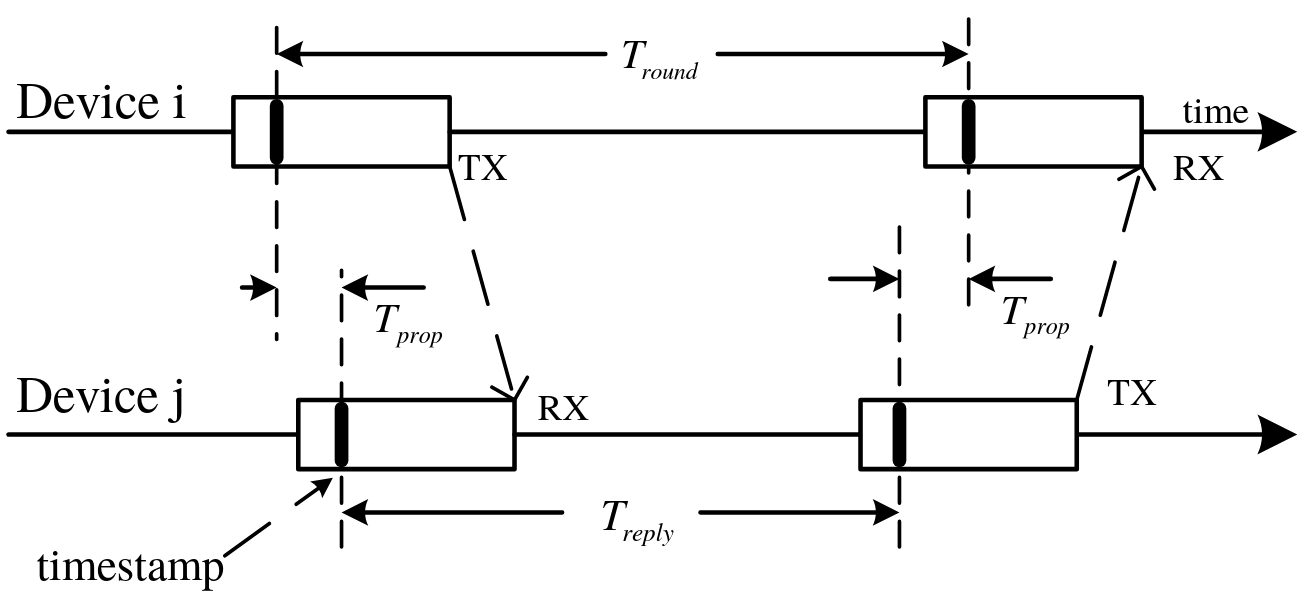
\includegraphics[width=0.7\linewidth]{Images/Related-Work/Single-Sided-Two-Way-Ranging-SS-TWR-5.png}
	\decoRule
	\caption[Illustration of Single-sided Two-way ranging]{Illustration of Single-sided Two-way ranging \cite{uwb-imu-gps1}}
	\label{fig:SS-TWR}
\end{figure}

τυπική απόκλιση = 0.1m
\begin{gather*}
    d_{ij} = \frac{1}{2}(T_{round} - T_{reply}) \times c = \norm{r_i - r_j} + n_{UWB}, \quad with \quad n_{UWB} \sim N(0, \sigma^2_{UWB}) 
\end{gather*}

Και ότι το ένα μπορεί να μεταφέρει τις πληροφορίες του στο άλλο

UWB module is set to operate at a rate of 100Hz

Each measuring interval
	dij calculate
	transmit to other nodes

% GPS
NEO-M8N GPS 5Hz.

\begin{gather*}
	r_{i,j} = r_{i, GPS} - r_{j, GPS} = r_{ij} + n_{GPS} \\
\end{gather*}


\begin{figure} [H]
	\centering
	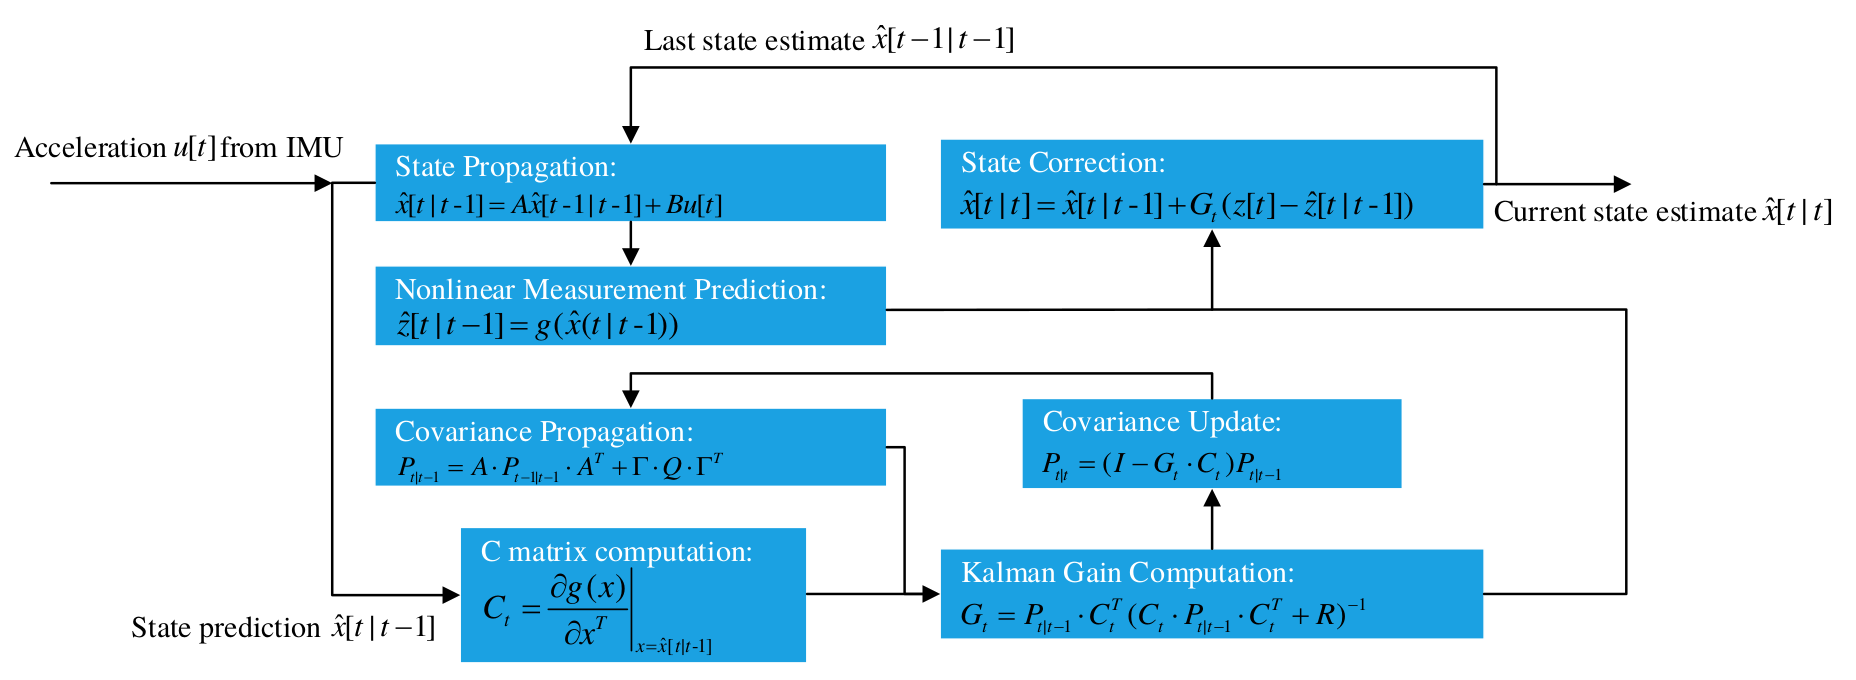
\includegraphics[width=\linewidth]{Images/Related-Work/Data-preprocessing-work-flow-using-EKF.png}
	\decoRule
	\caption[Data preprocessing work flow using EKF]{Data preprocessing work flow using EKF\cite{uwb-imu-gps1}}
	\label{fig:Data-preprocessing-work-flow-using-EKF}
\end{figure}

Θεωρούν το σύστημα ως ένα γράφο το οποίο 
το σημείο στο οποίο το σύστημα σταθεροποιηθεί θεωρείται ότι είναι το η γεωμετρία τοπολογίας των nodes
ενώ θεωρούν το σύστημα ως rigid body 

estimation problem into a non-convex optimization problem



small distance estimation error (within 0.4 m) while maintaining low
computational load

% 

of UWB pulses transmission and reception [1], and has an accuracy of less
than 10 cm UWB signals are particularly suitable for localization systems due to their high
accuracy as well as the ability to operate in Non-Line-of-Sight (NLOS)
it provides a channel for data communication and supports data transfer at a rate up to 6.8
Mbps.

First we
incorporate the UWB and the IMU measurement to reject the ranging outlier and recover the
distance between neighbors when ranging failure occurs, next we use these distance estimations
to construct a rigid body composed of these moving nodes and edges of certain length by finding
the global minimum of a non-convex function, finally the orientation of the rigid body system
is calculated using GPS coordinates of several nodes.

% ----------------------------------------------------------------

\begin{figure} [H]
	\centering
	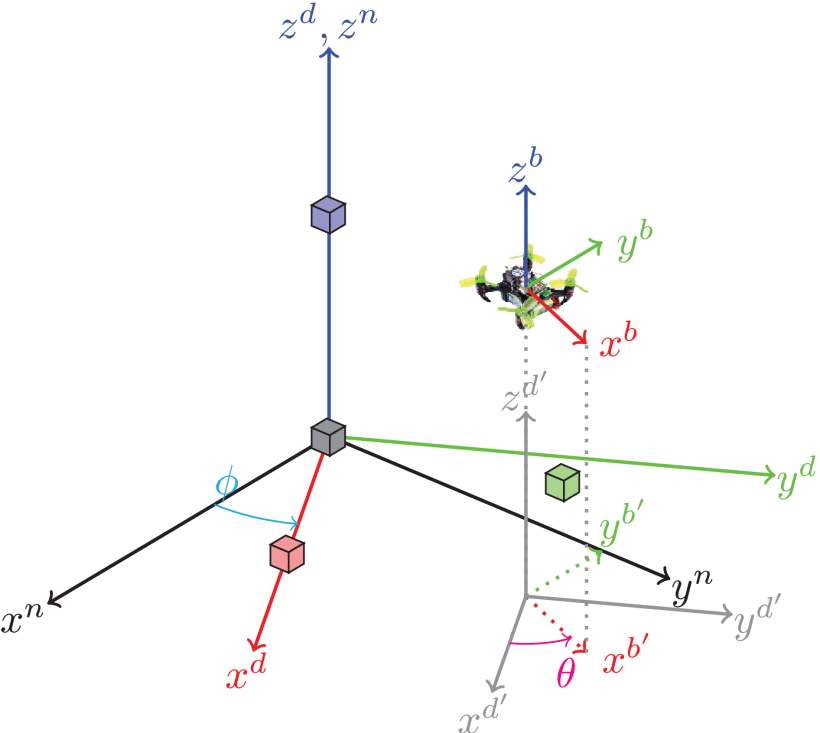
\includegraphics[width=0.6\linewidth]{Images/Related-Work/body-frames.png}
	\decoRule
	\caption[Important coordinate frames]{Important coordinate frames as shown on \cite{uwb-imu-gps2} DecaWave frame (d), Navigation frame (n), the body frame (b), the translated DecaWave frame ($d_0$) and the projected body frame ($b_0$)}
	\label{fig:Important-coordinate-frames}
\end{figure}
LPS methods based on Ultra-Wide Band (UWB)

Local Ad-hoc Positioning and Landing
System (LAOLa)

Local Positioning System (LPS)


Components-Off-The-Shelf (COTS)
Radio based
such as Radio Fre-
quency Identification (RFID) [9], WiFi [10], Zigbee [11] and
Ultra-Wideband (UWB)
% \begin{gather}
        
% \end{gather}

% \begin{gather}
        
% \end{gather}


% Some systems have been deployed and tested in real-life scenarios, while others remain theoretical approaches
% \cite{10.5555/3400306.3400339}
\cite{6907551}
% \cite{8355093}
% \cite{PMID:33348720}
% \cite{article5}
% \cite{inproceedings}
% \cite{inproceedings2}
% \cite{8453331}
% \cite{4967999}
\cite{inproceedings51}
% \cite{trilateration-application1}
% \cite{Qi_2020}


% \section{Demo: In-flight Localisation of Micro-UAVs using Ultra-Wide Band}

% IEEE 802.15.4-2011 

% distance measurement with a precision down to 10 cm within
% a 250 m range

% It combines good obstacle penetration, and
% resilience to both multi-path effects and interference from
% other wireless technologies
% Symmetrical Double-
% Sided Two-Way Ranging 

% Local Positioning System (LPS) 




% This should be the last section
\section{Thesis Approach}
TODO: As last section of this chapter
